\section{Introduction}\label{intro}
\begin{figure}[t]
\begin{subfigure}{0.49\linewidth}
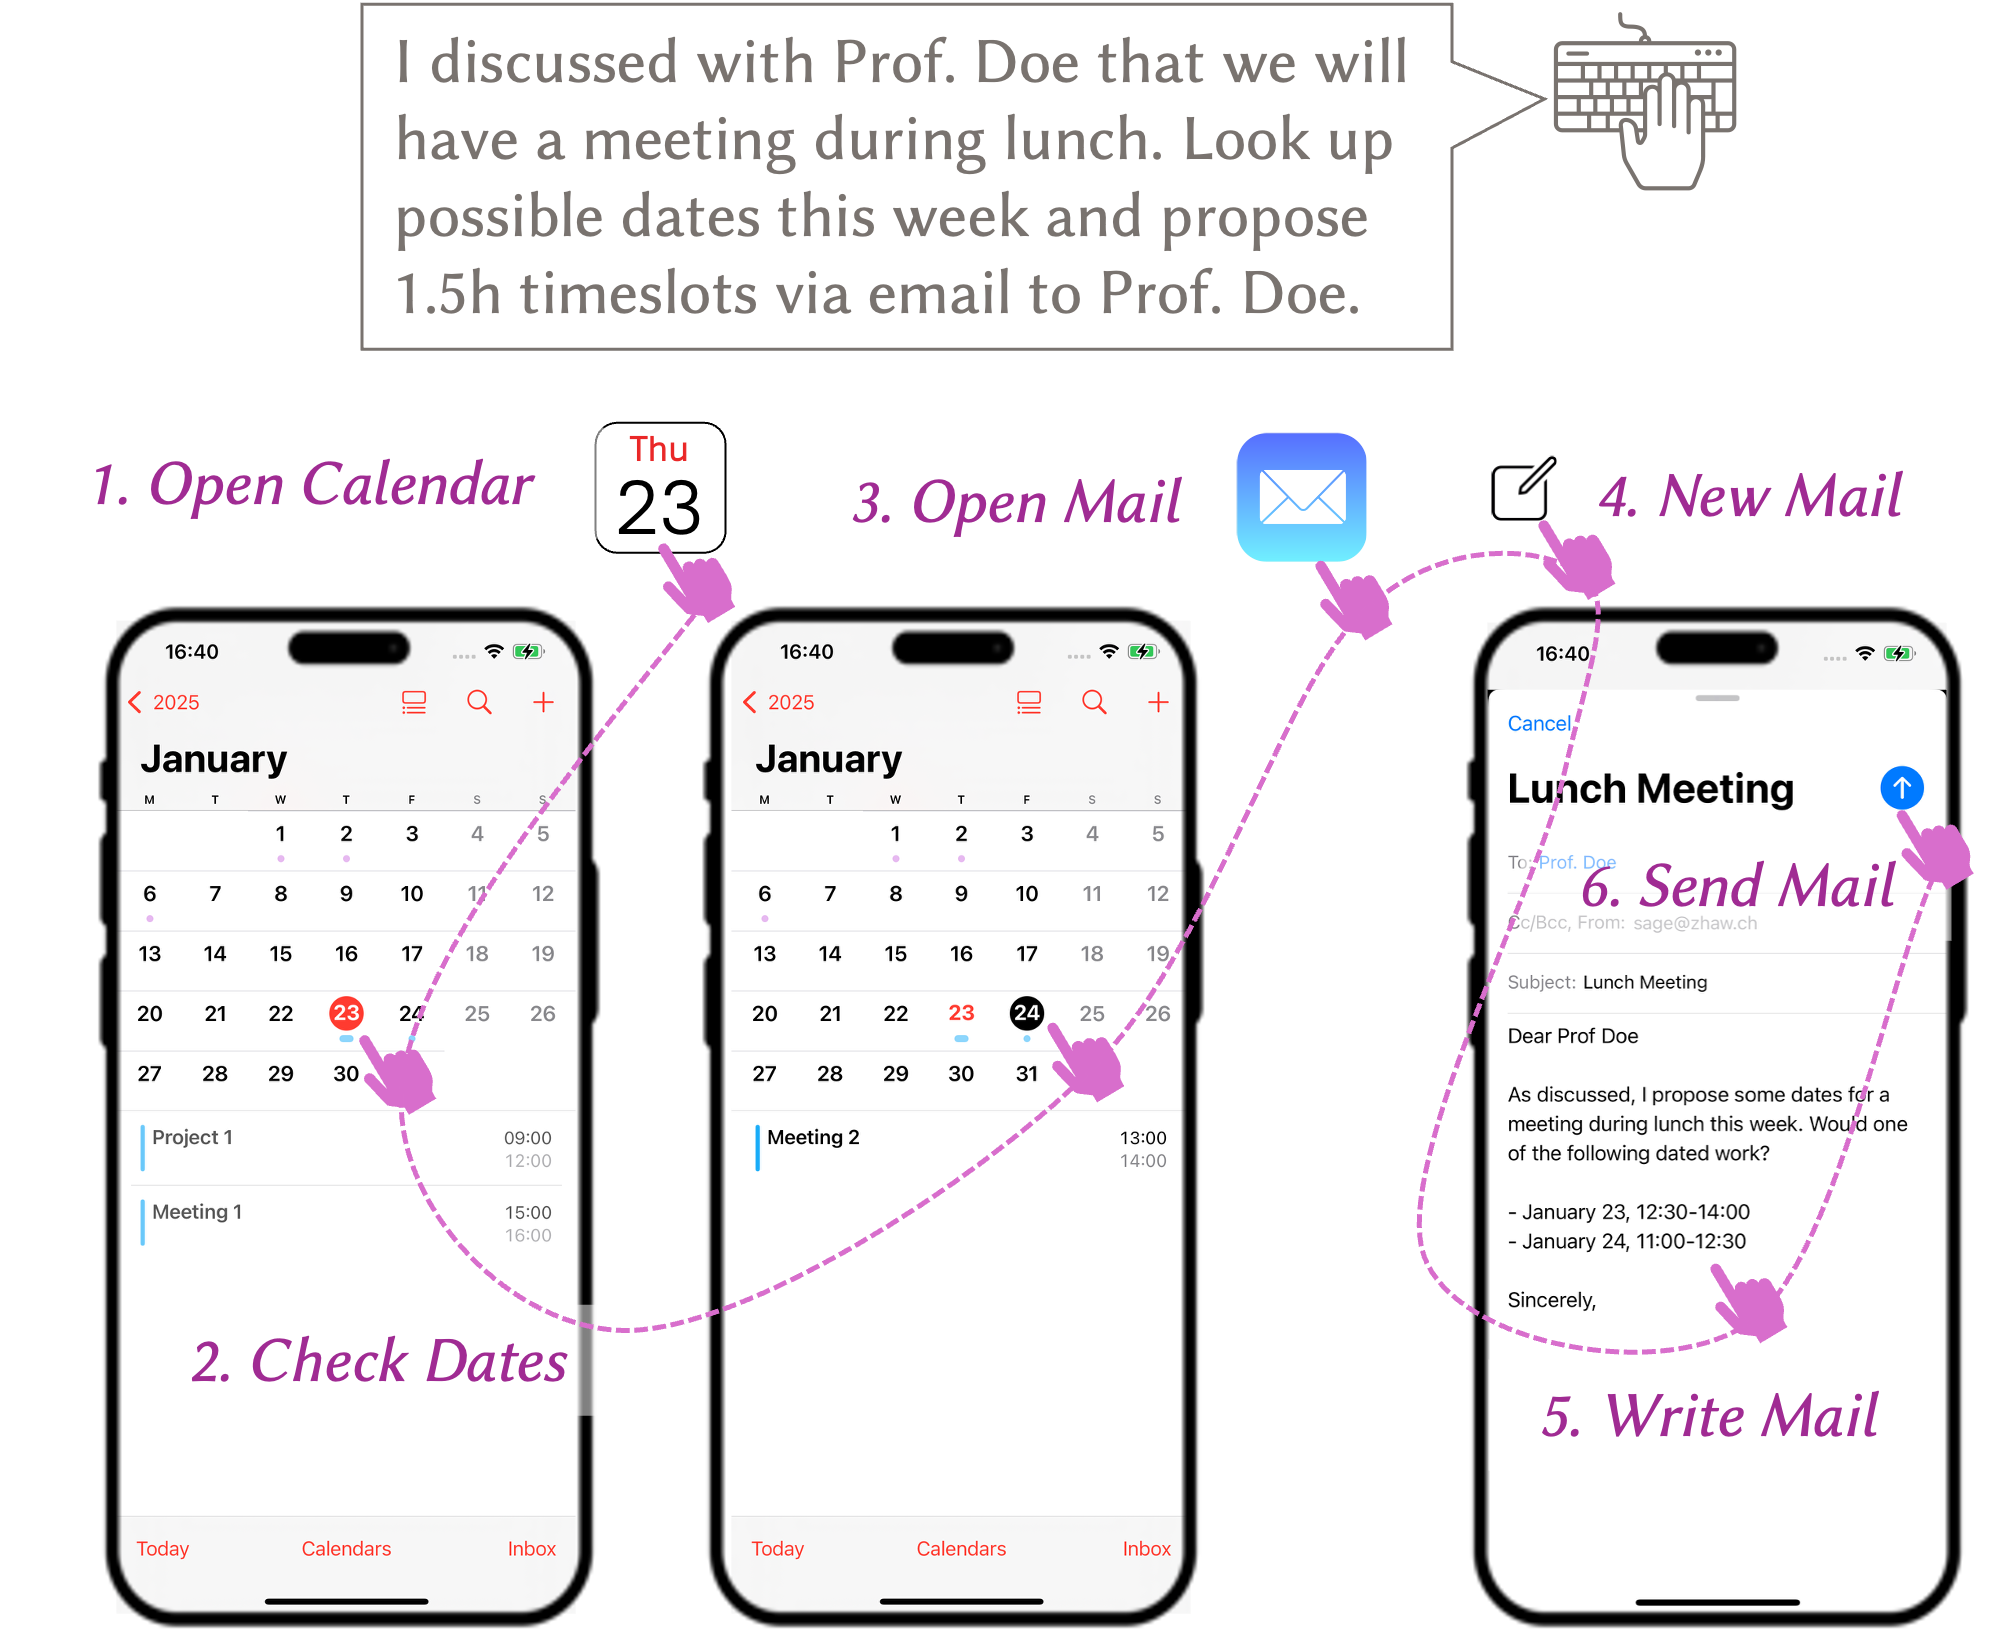
\includegraphics[width=\linewidth]{figures/ACU_example.png}
\caption{Example of a computer use task.}
%\Description{ A text bubble at the top shows the instruction to the agent: ``Look up possible dates this week and propose 1-5h timeslots for this week via mail to Prof. Doe.'' The agent then performs a sequence of six steps illustrated on three smartphone screenshots. Step 1: The agent opens the calendar app. Step 2: The agent checks available dates in the calendar. Step 3: The agent opens the email app. Step 4: A new email is created. Step 5: The agent writes an email suggesting meeting times. Step 6: The email is sent.  Arrows connect each step sequentially.
%}
\label{fig:ACU-example}
\end{subfigure}
\hfill
\begin{subfigure}{0.49\linewidth}
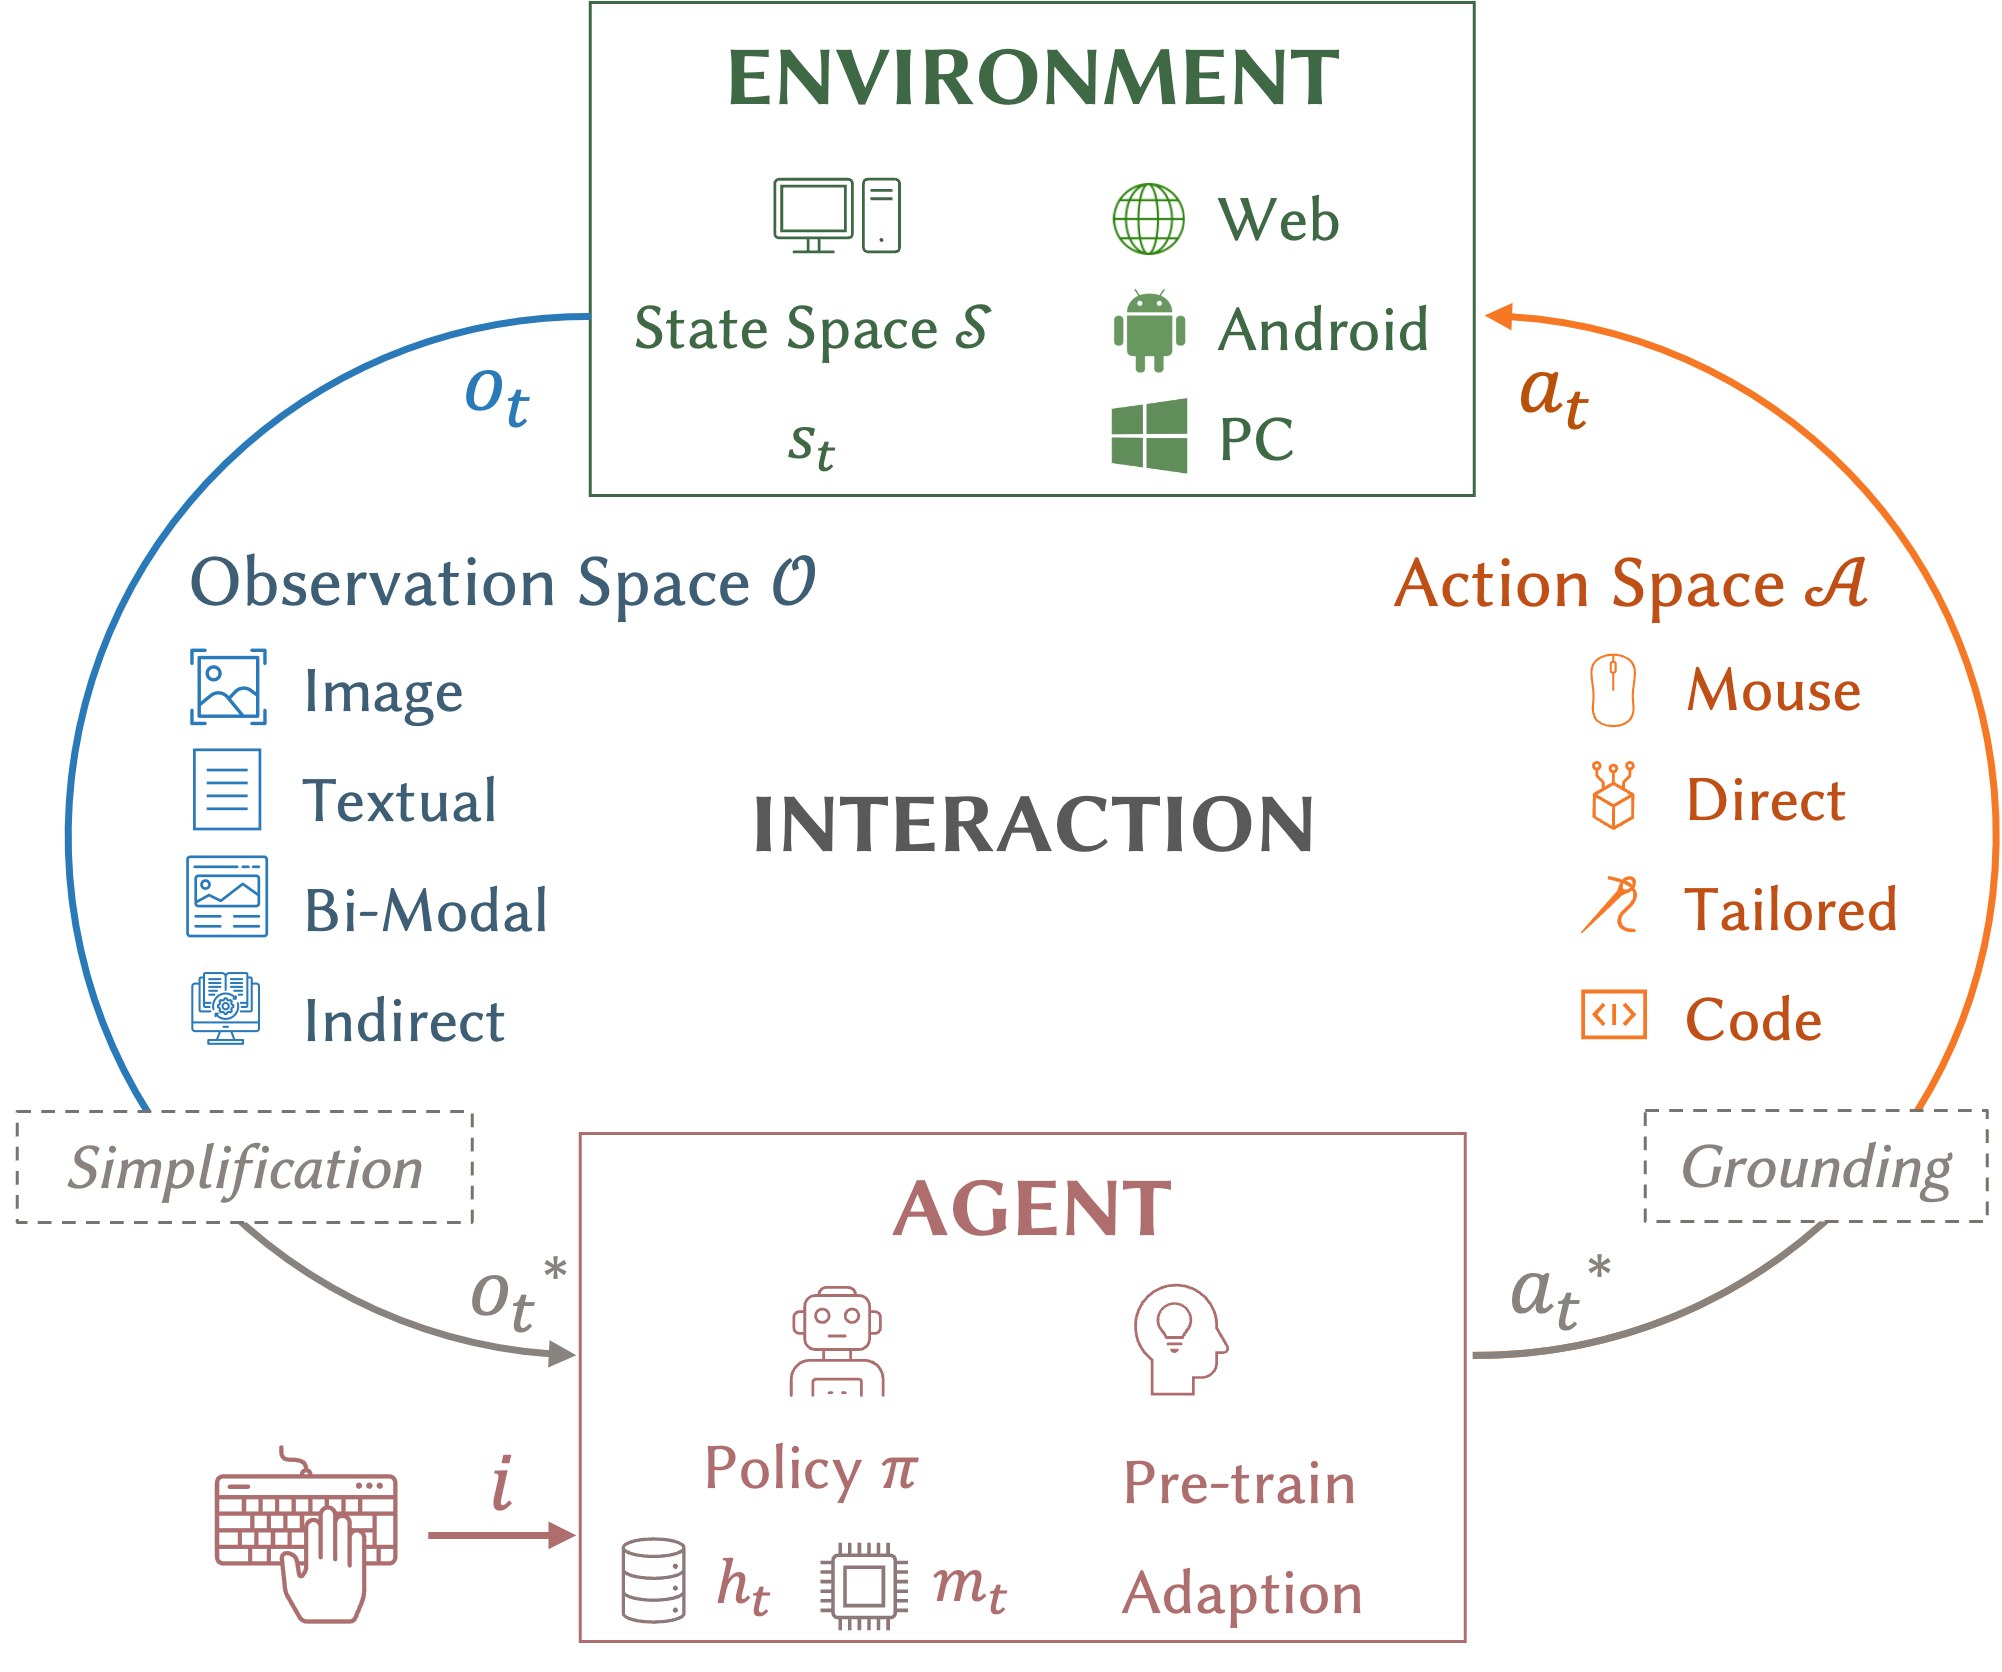
\includegraphics[width=\linewidth]{figures/ACU_taxonomy.png}
\caption{Proposed taxonomy.}
%\Description{
%A conceptual diagram showing the taxonomy of autonomous computer use (ACU) systems. At the top is the computer environment (which comprises the platforms  Web, Android, and PC, along with a state space)) and at the bottom is the agent.
%On the left is an arrow labeled as observation space, going from environment to agent. It comprises four modes: image, textual, bi-modal, and indirect observations. On the right an arrow going gtom agent to envrionment labeled as action space and listing mouse, direct, tailored, and code.}
\label{fig:ACU-taxonomy}
\end{subfigure}
\caption{
Overview: (a) An example of a task for an ACU: A user specifies a task (``propose meeting dates by email'') and the agent executes it.
(b) We structure the literature on ACUs based on three key \emph{perspectives} corresponding to the main differentiating aspects:
(1) The shared \emph{domain} properties across computer environments (e.g., Web, Android).
(2) The means of \emph{interaction} between the agent and the environment as manifested in the observation and action spaces.
(3) The \emph{agent} components: how an agent acts through a policy $\pi$ while tracking the past in memory and how an agent learns to act.}
\Description{Example of a typical task and conceptual taxonomy of ACU systems. In the left subfigure, a user instruction is shown in a text bubble at the top of the image: ``Look up possible dates this week and propose 1.5h timeslots via email to Prof. Doe.'' Below, a sequence of six steps is illustrated using three smartphone screenshots connected by arrows. The steps include opening a calendar app, checking available dates, switching to the email app, composing a message with proposed times, and sending the email. This visual sequence highlights the agent's execution of high-level user intent via low-level app interactions. In the right subfigure, a conceptual taxonomy diagram depicts the structure of ACU systems. At the top, the computer environment includes platforms such as Web, Android, and PC, along with their corresponding state spaces. Observation flows from environment to agent and is categorized into image-based, textual, bi-modal, and indirect observations. Action flows from agent to environment and is categorized into mouse interactions, direct input, tailored mechanisms, and code execution.}
\label{fig:intro}
\end{figure}

AI agents operate by perceiving their environment and selecting actions to achieve predefined goals \citep{mnih_playing_2013}.
This agent-based paradigm, popularized in the 1990s \citep{schmidhuber1990line, 10.1145/122344.122377, russell_artificial_2022}, has shown success across domains such as robotic control \citep{yang_data_2020}, game playing \citep{baker_video_2022}, and autonomous driving \citep{grigorescu_survey_2020}.
A growing class of agents extends this paradigm by allowing users to define goals in natural language \citep{ouyang_training_2022}. These instruction-based agents interpret textual instructions and autonomously act in complex environments to fulfill them.

One promising application of instruction-based agents is computer use, where agents control software through computer interfaces originally designed for humans. These agents automate tasks such as scheduling, browsing, or document editing by interacting with digital platforms via simulated inputs such as mouse clicks or touchscreen gestures.
For instance, a user could instruct an agent embedded in a smartphone to propose meeting dates and send them via email. The agent would then operate the phone through simulated touch actions to fulfill the request, as illustrated in \cref{fig:ACU-example}.
We refer to this class of agents as \textbf{agents for computer use (ACUs)}.

\begin{figure}
    \centering
    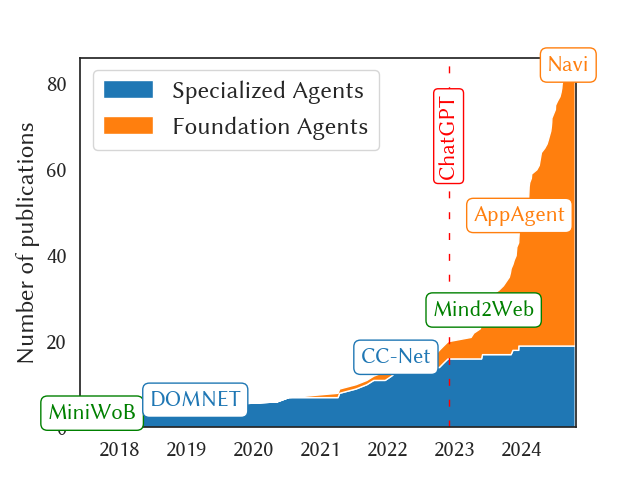
\includegraphics[width=0.6\linewidth]{figures/data/timeline_new.png}
    \caption{ACU publications over time. Boxes highlight seminal milestones. The advent of ChatGPT marks a shift from RL-focused agents to those primarily relying on foundation model reasoning.}
    \Description{
    Area chart showing the absolute number of publications per year from 2018 through 2024, separated by agent type. Differently colored areas distinguish specialized agents from foundation-model-based agents, with a legend identifying each. Key milestones, such as influential papers and dataset releases, are highlighted using boxed annotations along the timeline. A vertical red dashed line marks the launch of ChatGPT in late 2022, after which the number of publications on foundation-model-based agents rises sharply  (from about $20$ to over $80$ publications), overtaking specialized agents. The transition indicates a field-wide shift in research emphasis.}
    \label{fig:timeline-new}
\end{figure}

Early research on ACUs focused primarily on the learning methodology, particularly reinforcement learning (RL) techniques \citepeg{branavan_reinforcement_2009,jia_dom-q-net_2019,humphreys_data-driven_2022}.
Recently, a shift toward integrating foundation models, such as large language models (LLMs) and vision-language models (VLMs) (see \cref{sec:conceptional_view}), has accelerated progress, significantly enhancing reasoning capabilities and enabling ACUs to tackle increasingly complex tasks \citep{wei_emergent_2022,kim_language_2023}.
This transition has stimulated research activity, reflected in a strong increase in publications in the field (see \cref{fig:timeline-new}).

Concurrently, commercial prototypes of instruction-based agents for computer use have begun to emerge \citepeg{anthropic2024computeruse, google2024project, venturebeat2025openai}. However, despite this momentum, ACUs remain limited in their generalization, robustness, and planning abilities, achieving almost six time lower success rates than humans due to the inability of handling dynamic UI changes, switching between multiple software applications, or errors in dense UI environments such as spreadsheets \citep{xie_osworld_2024}.
To assess both the opportunities and barriers, we conduct a broad survey of ACUs across domains, learning strategies, and modalities. This survey complements the existing body of literature with a comprehensive taxonomy grounded in established intelligent agent theory \citep{russell_artificial_2022,sutton_reinforcement_2018}, enabling a holistic and technology-agnostic analysis of the ACU landscape (see \cref{fig:ACU-taxonomy} for an overview).

Applying this taxonomical framework to current research, we identify several critical research gaps.
First, many agents rely heavily on structurally inconsistent observations (e.g., unrealistically sanitized HTML), limiting their ability to generalize and scale to real-world applications.
Second, current learning strategies are costly and inefficient, often relying on simulations, requiring substantial labeled data, or struggling to adapt to specific environments.
Third, agents have a very limited ability to plan and execute complex multi-step tasks reliably.
Fourth, existing benchmarks focus on real-world perception but lack sufficient task complexity to fully assess agent capabilities.
Fifth, non-standard evaluation practices hinder meaningful comparison across different publications.
Sixth, a mismatch exists between the assumptions regarding ACUs and their operational environments made during research and the actual conditions encountered during real-world deployment.

To address these challenges, we propose several directions.
Observing and acting on uniform visual inputs provides more robust generalization than observing inconsistent textual inputs, e.g., HTML content.
To overcome inefficiencies in learning, we highlight the need for cost-effective strategies and discuss promising directions for more scalable adaptation.
To improve planning capabilities, we suggest exploring advances in reasoning models and integrating robust planning algorithms.
To close the gap in benchmarking ACUs, we advocate for the development of datasets that better capture task complexity alongside real-world perception.
To enable meaningful evaluation, we assert that the task success rate following standardized measurement practices should become the norm for comparing agent capabilities.
Finally, to bridge the gap between research assumptions and real-world conditions, we identify several key discrepancies and propose research directions to address them.

This survey aims to foster advancements in the field of ACUs by providing a principled and comprehensive overview of the domain. Specifically, our contributions are as follows: (1) The introduction of a comprehensive taxonomy for ACUs, (2) the classification of $\numagents$ ACUs and $\numdatasets$ datasets within this framework, (3) the identification of six critical research gaps, and (4) the proposal of strategic directions to address these challenges.


\subsection{Relation to Other Surveys}
In contrast to existing surveys, our review examines ACUs from a technology-agnostic perspective and introduces a unifying framework that bridges diverse domains, methodologies, and technologies.
This broader scope allows us to introduce a novel, unifying taxonomy for ACUs that is compatible across a wide range of agent types ---something previous work could not realize due to their limited scope. Specifically, existing surveys have the following limitations:

\begin{description}
    \item[Limitation in learning strategies:] \citet{zhang_large_2024} and \citet{wang_gui_2024} focus only on computer use for foundation-model-based agents, without discussing other learning frameworks such as pure reinforcement learning as the core principle of design. In contrast, 
    other surveys \citepeg{arulkumaran_deep_2017, moerland_model-based_2023} focus only on general reinforcement learning-based agents.

    \item[Limited scope within computer use:] 
    % \citet{zhang_large_2024} and \citet{wang_gui_2024} review computer use only for foundation-model-based agents, not discussing other learning frameworks such as reinforcement learning as the core principle of design.
    \citet{wu_foundations_2024} discuss only mobile agents, neglecting other computer domains.
    While their survey provides a comprehensive review of some aspects of computer use, it focuses on a specific subpart of the field. To discuss future research directions comprehensively, it is important to analyze the field as a whole.
    \item[Lack of computer use specificity:]
    % Some surveys \citepeg{arulkumaran_deep_2017, moerland_model-based_2023} focus on general reinforcement learning-based agents.
    % Other surveys \citepeg{wang_survey_2024,li_multimodal_2024} review general foundation-model-based agents.
    % While these 
    Other reviews \citepeg{arulkumaran_deep_2017, wang_survey_2024} provide a comprehensive overview of agents based on a specific technology but do not focus on the domain of computer use and all its intricacies.
    \item[Adjacent research areas with limited relevance for agentic computer use:]
    Another set of surveys \citepeg{yu_vision-based_2023, li_gui_2023} concentrate on related topics, such as GUI testing, but do not cover agent-based interactions.
    Other reviews \citepeg{syed_robotic_2020, asatiani_robotic_2020} focus on robotic process automation using scripted software robots (also called agents) to automate predefined workflows.
\end{description}

\citet{gao_generalist_2024} provide a valuable overview with a similar scope. In contrast, we go considerably deeper into key aspects, offering a more comprehensive analysis and novel insights, based on a taxonomy built upon existing intelligent agent theory \citep{russell_artificial_2022,sutton_reinforcement_2018} that is useful to find related work down to intricate questions of agent design. We posit that a comprehensive and in-depth review of the field is essential to systematically uncover the limitations of current agents and identify how diverse technologies and methodologies can inform one another to advance the state of the art.

\subsection{Survey Methodology}
\begin{figure}[ht]
    \centering
    \begin{tikzpicture}[
        node distance=0.8cm and 0.8cm,
        font=\footnotesize,
        % Styles
        process/.style={rectangle, minimum width=2.2cm, minimum height=1cm, text centered, draw=black, fill=blue!5, rounded corners},
        % Style for the Criteria Box (Dashed, indicating input/control)
        criteria/.style={rectangle, minimum width=2.2cm, minimum height=0.8cm, text centered, draw=black, dashed, fill=yellow!5, rounded corners, font=\scriptsize},
        % Rotated Trapezium for Final Set
        finalnode/.style={trapezium, shape border rotate=270, trapezium angle=60, minimum height=1.8cm, minimum width=1.1cm, text centered, draw=black, fill=green!5, inner sep=1pt, align=center},
        arrow/.style={thick, ->, >=stealth}
    ]
    
    \node (sources) [process, text width=2.5cm] {Initial collection};
    
    % Phase 2: Publication Selection
    \node (screen) [process, right=of sources, text width=2.5cm] {Publication selection};
    
    % Selection Criteria (Input to Phase 2)
    \node (criteria) [criteria, above=0.6cm of screen, fill=white, text width=2.5cm] {Selection Criteria}; % \\(DL, Comp. Use, Common Appl.)
    
    % Phase 3: Snowballing (Loop)
    \node (snowball) [process, below=0.6cm of screen, text width=2.5cm] {Snowballing};
    
    % Final Set (Rotated Style)
    \node (final) [finalnode, right=0.6cm of screen] {Final\\Set}; %\\($N{=}\numpapers$)
    
    % Split Categories (Stacked)
    \node (agents) [process, right=0.8cm of final, yshift=0.6cm, minimum width=2.2cm, fill=orange!5, minimum height=0.7cm] {Agents ($N{=}\numagents$)};
    \node (data) [process, right=0.8cm of final, yshift=-0.6cm, minimum width=2.2cm, fill=orange!5, minimum height=0.7cm] {Datasets ($N{=}\numdatasets$)};
    
    % Phase 4: Data Analysis and Synthesis
    \node (synthesis) [process, right=0.5cm of agents, yshift=-0.6cm, text width=2.5cm, minimum height=1.9cm]
    {Data Analysis and Synthesis};
    
    \draw [arrow] (sources) -- (screen);
    \draw [arrow] (criteria) -- (screen); % Arrow from criteria to selection
    \draw [arrow] (screen) -- (final);
    
    % Snowball loop arrows
    \draw [arrow] (screen.south) -- (snowball.north);
    \draw [arrow] (snowball.west) -- ++(-0.3,0) |- (screen.west);
    
    % Split arrows
    \draw [arrow] (final.east |- agents.west) |- (agents.west);
    \draw [arrow] (final.east |- data.west) |- (data.west);
    
    % Synthesis arrows
    \draw [arrow] (agents.east) -- (synthesis.west |- agents.east);
    \draw [arrow] (data.east) -- (synthesis.west |- data.east);

    \end{tikzpicture}
    \caption{Visual overview of the survey methodology phases, detailing the selection logic and synthesis process.}
    \Description{
    A horizontal flowchart illustrating the four-phase survey methodology. The process flows from left to right. It begins with Phase 1: Initial Collection, which leads into Phase 2: Publication Selection. Phase 2 inputs include specific Selection Criteria (Deep Learning, Computer Use, Common Applications) and an iterative feedback loop with Phase 3: Snowballing. The output of Phase 2 is a Final Set of papers (N papers). This final set branches into two categories: Agents (N agents) and Datasets (N datasets). Both categories feed into the final step on the right, Phase 4: Data Analysis and Synthesis.
    }
    \label{fig:methodology}
\end{figure}

The field of ACUs is fragmented and lacks a unified terminology, making a classic systematic review infeasible. We therefore employed an iterative, semi-structured collection process combining expert knowledge with snowball sampling techniques. As visualized in \cref{fig:methodology}, our methodology comprised the following phases:

\begin{description}
    \item[Initial collection:] Based on domain expertise and exploratory keyword-based searches, we compiled an initial set of candidate publications. Given the rapid evolution of this domain, we included both peer-reviewed and preprint works to reflect the state-of-the-art. 
    We conducted a semi-structured search using Google Scholar and Semantic Scholar, combining keywords such as ``AI agent'', ``LLM/LVM agent'', and ``computer use''. We only collect the papers from the last $7$ years (2018-2024).
    \item[Publication selection:] After initial collection, we filtered the literature and included publications after carefully reviewing their titles, abstracts, and additional parts of their content for fit, using the criteria catalog described below. The selection was conducted by two researchers independently, followed by a consensus discussion. Since some publications are preprints, we evaluated them by using domain knowledge and checked their consistency with emerging trends to mitigate quality concerns.
    \item[Snowballing:] We used backward snowballing for adding references and forward snowballing for determining saturation: For each selected publication, we analyzed its references (backward), and for randomly selected works, we analyzed citations (forward) and checked whether additional relevant works could be identified. We iteratively repeated this process until no additional relevant papers emerged, ensuring thematic saturation.
    \item[Data Analysis and Synthesis:] To develop the taxonomy, we employed an inductive approach. We extracted key attributes from the final set of papers (e.g., input modalities, action spaces, evaluation metrics) and grouped them into high-level dimensions. This process was iterative; as new properties emerged during data extraction, the taxonomic dimensions were refined to ensure they covered both agent architectures and dataset characteristics comprehensively.
\end{description}

The selection criteria for the collection process for both agent and dataset papers are defined as follows:


\begin{description}
    \item[Deep learning focus:]
        We only included agents utilizing deep learning for computer use, excluding traditional rule-based systems.
    \item[Computer use focus:]
        We distinguish between passive advice and active execution. We exclude instruction-based agents (chatbots) that access external tools but only provide text advice or instructions for a human to follow \citepeg{yang_gpt4tools_2023,tang_toolalpaca_2023,li_towards_2024,guo_stabletoolbench_2024,qin_toolllm_2024}. 
        In contrast, we include agents that generate executable code (e.g., Python/Selenium scripts). Although these agents output text (code), this code acts as a dynamic action space that is executed by an interpreter to directly manipulate the interface, thereby satisfying our definition of autonomous computer use.
    \item[Common computer applications focus:]
        We exclude agents playing video games \citepeg{baker_video_2022, zhu_ghost_2023}, controlling server facilities \citepeg{ran_deepee_2019, fulpagare_optimal_2022}, coding agents \citepeg{ross_programmers_2023, qian_chatdev_2024} or software testing \citepeg{koroglu_qbe_2018, degott_learning_2019, pan_reinforcement_2020}.
        We only include datasets that provide instructions and require agents to fulfill these instructions through computer interactions.
\end{description}

The final set of publications was curated through a multi-stage screening process and agreement through team discussion to ensure comprehensive coverage of the field. Our selection criteria are prioritized by scholarly impact (high citations or benchmark leadership), representation of key application domains (e.g., Web, Android), and diverse coverage across taxonomic dimensions outlined in \Cref{fig:framework}.

From the identified publications, we classify $\numagents$ as ACU agents and $\numdatasets$ as computer use datasets. We deliberately separate these two categories in our analysis because they serve distinct roles in the ecosystem: agents represent the \textit{methodological solutions} and architectures, while datasets provide the \textit{evaluation environments} and benchmarks. Analyzing them separately allows us to derive specific taxonomies for architectural properties (e.g., learning paradigms, see Appendix \ref{appendix_A1}--\ref{appendix_A2}) versus environmental properties (e.g., observation spaces, see Appendix \ref{appendix_A3}).

Nevertheless, we note several limitations: (i) In our review, about 1/3 of the cited works are preprints. While they reflect emerging trends, they may lack validation and introduce concerns about quality. Readers should interpret these works cautiously; (ii) keyword search and manual screening, even when combined with snowballing, might have overlooked relevant papers; (iii) the focus on deep learning excludes traditional machine learning and rule-based approaches; and (iv) selection involves subjective judgment. To mitigate these limitations, we took several steps. For the inclusion of preprints, we cross-referenced findings with peer-reviewed literature when possible. To address potential gaps from keyword search and manual screening, we iteratively refined our search strategy and complemented it with citation tracking. Although our focus excluded traditional machine learning and rule-based approaches, we clearly defined this scope upfront to maintain consistency. Finally, to reduce subjective bias in selection, we employed a consensus-based review process, where disagreements were discussed and resolved collectively by multiple reviewers.

\subsection{Survey Structure}

Due to the developing nature of this field, individual ACUs that stand for important strands do not yet stand out; rather, many agents only employ certain aspects of what contributes to the full picture of ACUs. Hence, most subsequent chapters of this review put individual elements of the taxonomy at the center rather than individual ACUs, giving representative exemplary or specific ACUs as references for each aspect. A notable exception will be \cref{sec:learning_strategy}, where individual agents are most prominently portrayed, as it discusses their core development paradigm. Otherwise, a structuring of the field by agents can be found in the tables in the Appendix~\ref{sec:appendix_tables}. 

The survey is structured as follows: In \cref{sec:field}, we formalize the problem of agents for computer use and introduce respective terminology as a precursor to introducing the perspectives of the proposed taxonomy. Then, we look into each perspective in detail in the three subsequent chapters:
% In \cref{sec:approaches_overview}, we provide an overview of various agent architectures.
In \cref{sec:domain_view}, we discuss the composition of commonly used domains (\emph{domain perspective});
in \cref{sec:interaction_view}, we analyze the interaction between the agent and the environment through the observation and action space (\emph{interaction perspective}); 
in \cref{sec:conceptional_view}, we dissect the components of an agent, how an agent acts, and how an agent learns to act (\emph{agent perspective}). 
Then, in \cref{sec:datasets}, we summarize existing datasets used to train or evaluate agents, and we examine metrics and methodologies used to evaluate an agent's performance in \cref{sec:evaluation_agent}.
Finally, we conclude by summarizing our findings and providing directions for future research in \cref{sec:discussion_conclusion}.

To complement the main text, the Appendix provides several in-depth analyses:
In \cref{sec:appendix_trends}, we examine trends and distributions in the literature, including common choices of observation modalities, action spaces, and learning strategies;
\Cref{sec:img_vs_text,sec:code_generation_examples} contrast different observations and provide examples of code-based actions;
\Cref{sec:domain_view:nature,sec:considerations_production} discuss challenges in deploying ACUs, such as mismatches between environment properties assumed in research and found in real-world settings;
% Appendix \cref{} discusses challenges in deploying ACUs in practical settings;
\Cref{sec:appendix_tables} presents a structured overview of existing agents and datasets, classifying them according to our proposed taxonomy.